% -*- latex -*-
%%%%%%%%%%%%%%%%%%%%%%%%%%%%%%%%%%%%%%%%%%%%%%%%%%%%%%%%%%%%%%%%
%%%%%%%%%%%%%%%%%%%%%%%%%%%%%%%%%%%%%%%%%%%%%%%%%%%%%%%%%%%%%%%%
%%%%
%%%% This text file is part of the source of 
%%%% 'Parallel techniques'
%%%% by Ángel de Vicente, copyright 2019
%%%%
%%%% TO DO:
%%%%
%%%% basic-fortran.tex : basic fortran towards a first N-body implementation
%%%%
%%%%%%%%%%%%%%%%%%%%%%%%%%%%%%%%%%%%%%%%%%%%%%%%%%%%%%%%%%%%%%%%
%%%%%%%%%%%%%%%%%%%%%%%%%%%%%%%%%%%%%%%%%%%%%%%%%%%%%%%%%%%%%%%%

\Level 0 {Basic Fortran}
\label{sec:basic-fortran}

In this chapter we will just cover the basic concepts of Fortran. Fortran is a
complex language, so in this chapter we will only cover the surface of the
language, only the necessary minimum to be able to write a first implementation
of the N-body problem.

The following slides are taken from a 5-day intentive course on Fortran, given by the
University of Liverpool.

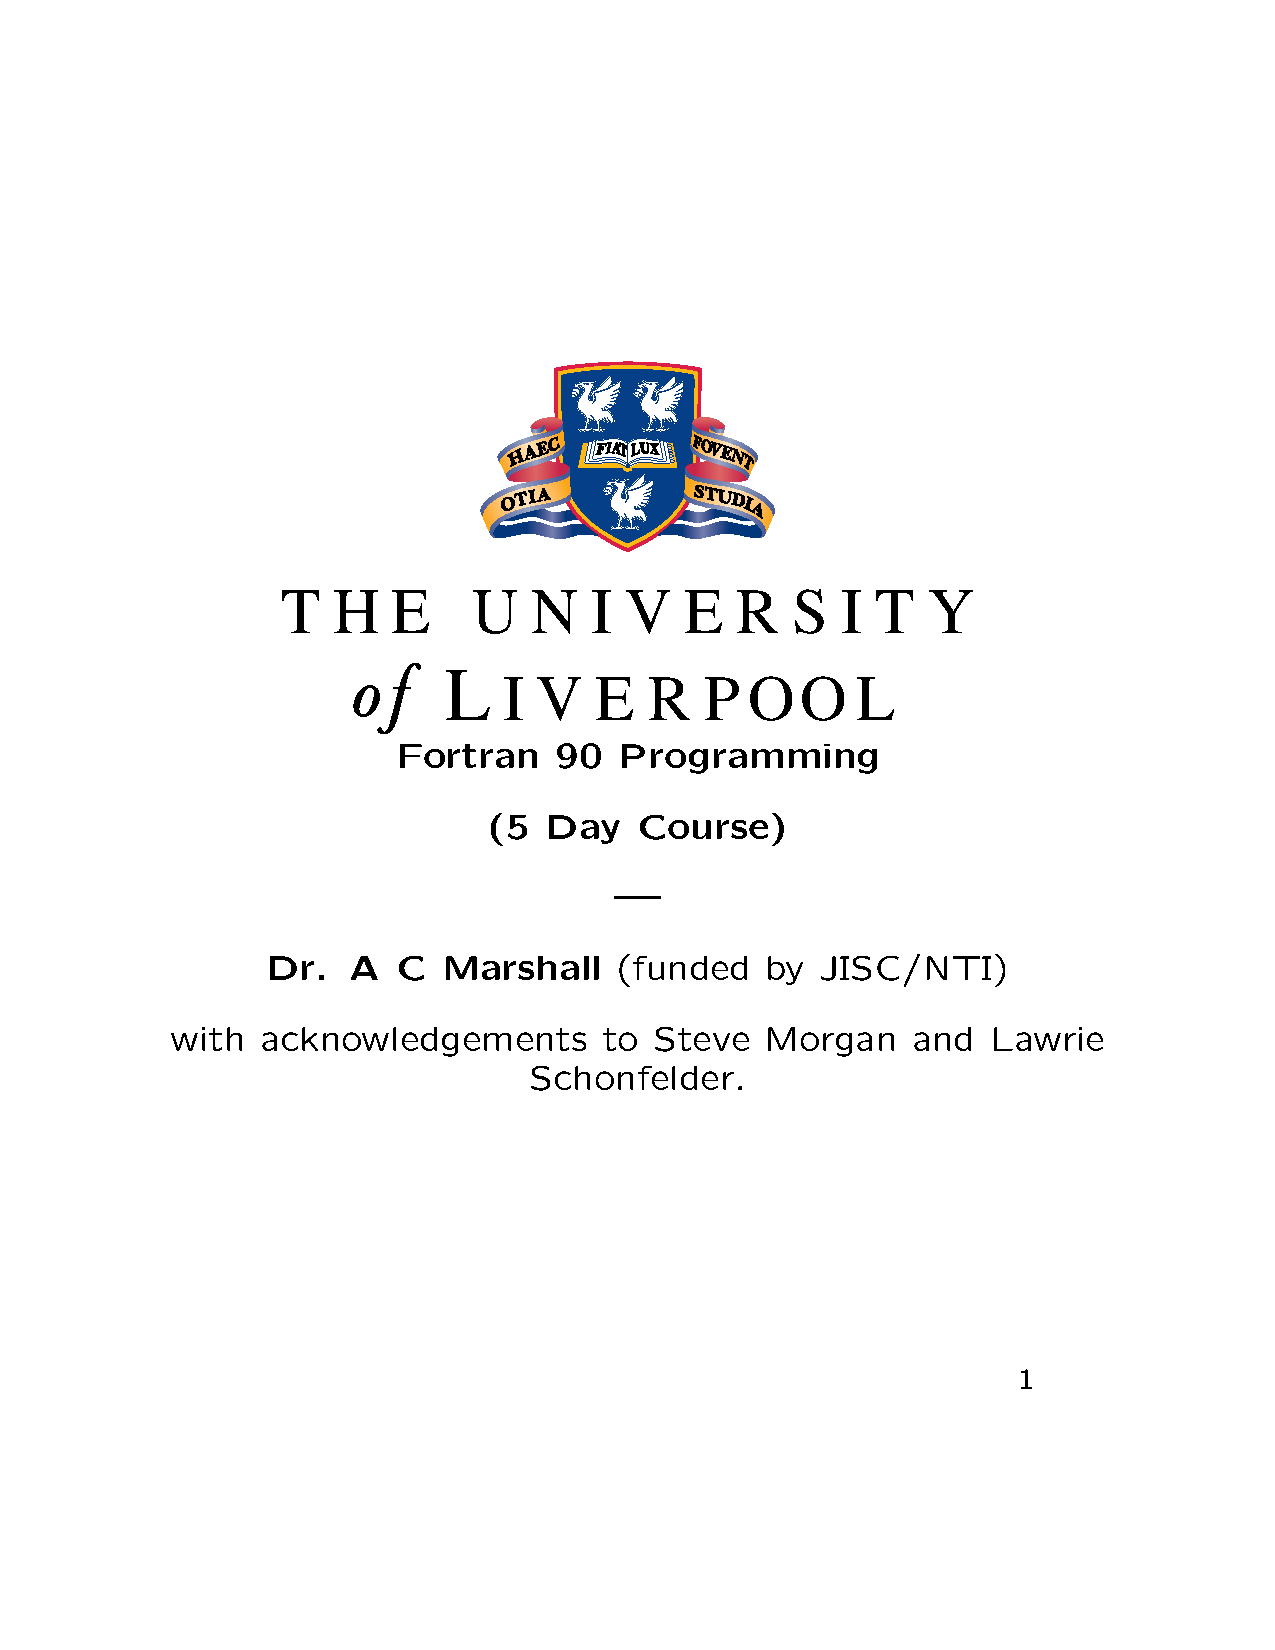
\includepdf[frame=true,scale=0.98,pages={1,3,6-8,10-13,15-21,23-36,38-39,41-54}]{graphics/CourseSlides_clase1.pdf}




